\documentclass{article}
\usepackage[english]{babel}
\usepackage{cancel}
\usepackage{tikz}
\usepackage{amsmath}
\usepackage{amsfonts}
\usepackage{amssymb}
\usepackage{graphicx}
\usepackage{subcaption}
\usepackage{caption}

\graphicspath{{./figs/}}

\title{Notes on Helix Fit}
\author{Kang, Byungmin}
\begin{document}
	\maketitle
	\section{Introduction to Helix Fit}
	Let us say, we want to determine a helical trajectory from a set of measured spatial points(or, hits). A point in a helical trajectory, $\mathcal H(c_x,c_y,r,z0,dz;\theta)$, can be represented by a parameter $\theta$ and five coefficients, which corresponds to the radius $r$, x and y of the center of the circle $c_x,c_y$, axis position at $\theta=0$ $z_0$, and helical pitch $dz$.
	
	To conduct a $\chi^2$ fit of the track from a set of measured spatial points(or, \textbf{hits}), we need to evaluate the distance of each point from the trajectory, estimate the pull by dividing it into spatial residual $\sigma$, and then sum up the square of the pulls to determine the $\chi^2$. Each hit comprise of three measurements, $\mathbf X_i \equiv (x_i,y_i,z_i)$. However, to define the distance between helical track and spatial point, \textit{we need to define a specific point}($\mathbf{h}_i$) by selecting specific parameter, $\theta_i$, in the helix($H(c_x,c_y,r,z0,dz;\theta)$) for each measurement $\mathbf X_i$. This point selection will be discussed in the next session. Selection of the point results in a \textit{loss of one degree of freedom, giving only two degrees of freedom for each hit}. Then, the summation for pull squared should have two spatial components. Our intuition says that, \textbf{radial}(along the plane where the circle lies) component and \textbf{vertical}(along the axis) component are the best choices.
	\begin{align}
		\chi^2 = \sum_i^n(\frac{\delta_{r,i}}{\sigma_{r,i}})^2 + (\frac{\delta_{V,i}}{\sigma_{V,i}})^2 - Cov(r,V)\frac{\delta_{r,i}}{\sigma_{r,i}}\frac{\delta_{V,i}}{\sigma_{V,i}}\label{chi2}
	\end{align}
	where $\delta_r$ and $\delta_V$ are the radial and vertical component squared, respectively, for the position difference $\mathbf{D}_i = \mathbf{h}_i - \mathbf{X}_i$, and $Cov(r,V)$ is the covariance between $\delta_r$ and $\delta_V$. 
	\section{Point Selection in Helical Track}
	To evaluate \eqref{chi2} properly, we need a good criteria to define $\mathbf{h}_i$. The simplest way is to get $\theta_i$ by minimizing
	\begin{align}
		\delta_i^2 &= (\mathbf h_i - \mathbf X_i)^2 \nonumber \\
		&=\underbrace{(c_x+r \cos\theta - x_i)^2+(c_y+r \sin\theta - y_i)^2}_{\delta_r^2} + \underbrace{(z_0 + dz\theta -z_i)^2}_{\delta_V^2}.\label{PoC}
	\end{align}
	This is known as \textit{Point of Closest approach}(PoC) method. However, with this definition, we have non-zero (anti) correlation between $r$ and $V$, arising from the minimizing condition:
	\begin{align}
		\frac{\partial \delta_i^2}{\partial \theta} = \frac{\partial \delta_r^2}{\partial \theta}+\frac{\partial \delta_V^2}{\partial \theta} = 0.\label{DifPoC}
	\end{align}
	In order to avoid this problem, we could define $\mathbf h_i$ by implying criteria other than \eqref{PoC} to avoid (anti) correlation between two variables from \eqref{DifPoC}. We can either minimize $\delta_r^2$ or $\delta_V^2$ only.
	
	If we minimize $\delta_V^2$, resulting $\theta$ from
	\begin{align}
		\frac{\partial \delta_V^2}{\partial \theta} = dz (z_0+dz\theta-z_i)=0\to \theta = \frac{z_0-z_i}{dz}\label{dV}
	\end{align}
	will be is extremely sensitive to small variance in vertical direction for tracks with low pitch angle($dz\to 0$), leading to high instability for $\theta_i$ selection, hence degrading the fitting result.

	Another choice, say \textit{Minimal Radial Distance}(MRD)\footnote{I can't find conventional name for this method} method is to minimize $\delta_r^2$, which would obviously be unstable for small radius ($r\simeq \sigma_r$). However, this is not the usual case because $r$ typically ranges from few hundreds to thousands of millimeters, while $\sigma_r < 10$ mm. Then, we have
	\begin{align}
		\frac{\partial \delta_r^2}{\partial \theta}& = -r(c_x+r\cos\theta-x_i)\sin\theta + r(c_y+r\sin\theta-y_i)\cos\theta=0\label{dR} \\
		\tan \theta& = \frac{\delta_y}{\delta_x}.
	\end{align}
	Figure \ref{Rep} illustrates the (a) PoC method and (b) MRD method. Note that, for small $dz$ tracks, \eqref{dV}$\simeq 0$ hence \eqref{DifPoC}$\simeq$ \eqref{dR} so that PoC and MRD becomes essentially similar.
	\begin{figure}[h]
		\centering
		\begin{picture}(400,140)
			\put(0,0){
				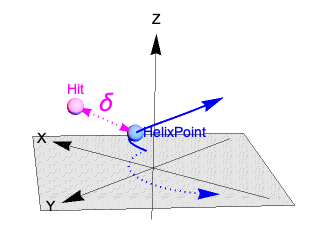
\includegraphics[width=200 pt]{Helix}
				\put(-180,120){
					\large (a)
				}
			}
			\put(200,0){
				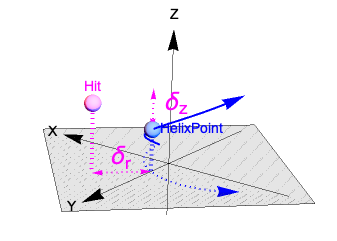
\includegraphics[width=200 pt]{Planar}
			\put(-180,120){
					\large (b)
				}
			}
		\end{picture}
		\caption{}\label{Rep}
	\end{figure}
	\section{Result Comparison in HypTPC}
		\begin{figure}[h]
		\centering
		\begin{picture}(400,180)
			\put(0,0){
				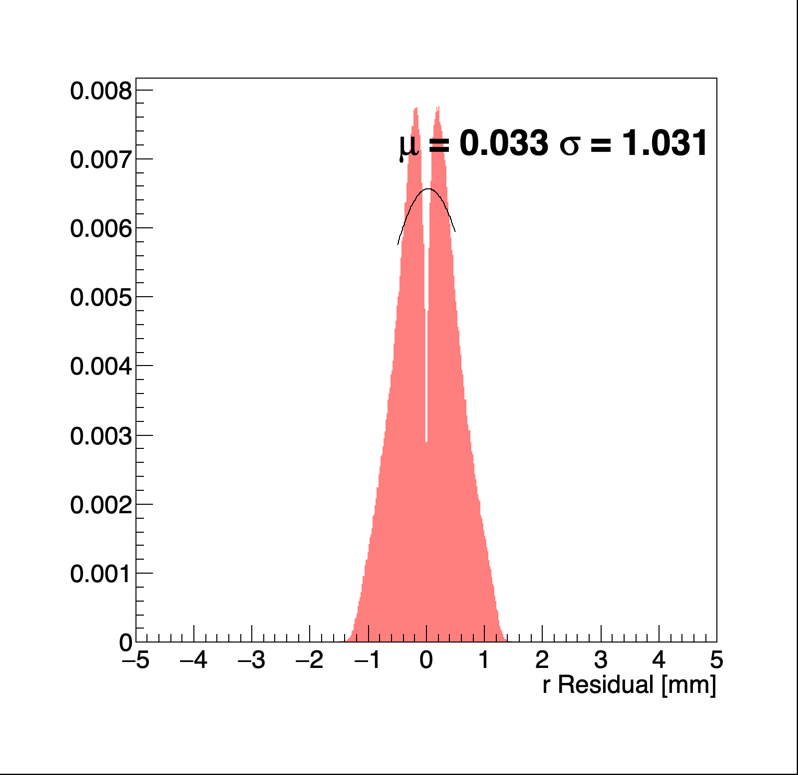
\includegraphics[width=200 pt]{ResR_Helix}
				\put(-160,150){
					\large (a)
				}
			}
			\put(200,0){
				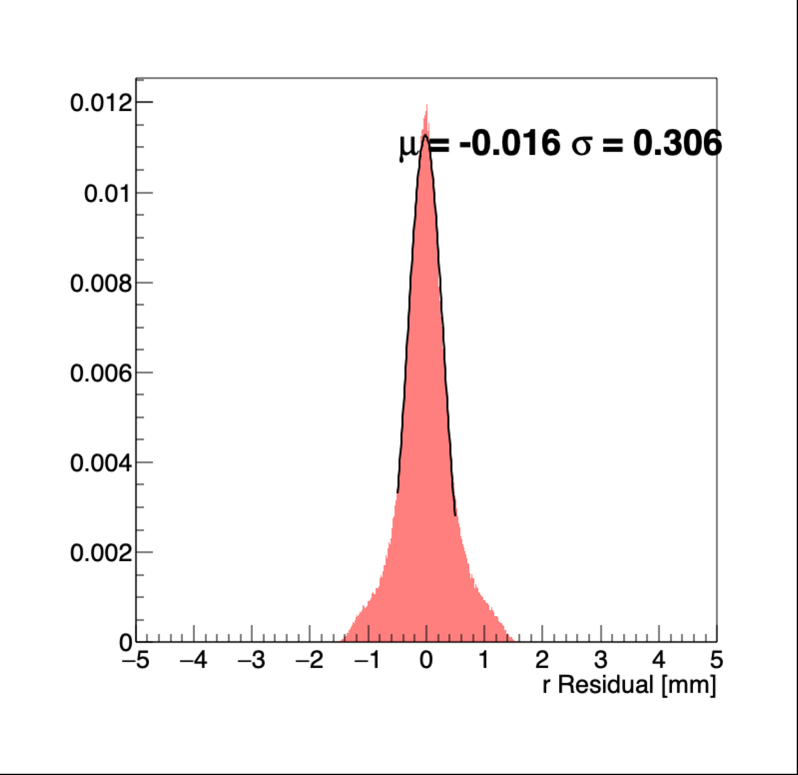
\includegraphics[width=200 pt]{ResR_Planar}
				\put(-160,150){
					\large (b)
				}
			}
		\end{picture}
		\caption{}\label{Resi}
	\end{figure}
	Figure \ref{Resi} shows the comparison of radial residuals between (a) PoC Method and (b) MRD method for scattered $\pi$s from $^{12}$C target, in 1T B-field. As discussed in the above section, PoC method minimizes $\delta_r^2+\delta_T^2$, hence $\delta_r$ may not be in minimum. As so we observe a dip structure in (a).
\end{document}
